\section{Feature Extraction from RGB and RGB-D Observations}\label{app:feature_extraction_from_rgb_and_rgbd_observations}

\autoref{app_fig:image_feature_extractor} shows a network architecture for the feature extractor that is used for RGB and RGB-D observations for \hyperref[subsec:comparison_of_2d_2_5d_3d_observations]{experiment~\ref*{subsec:comparison_of_2d_2_5d_3d_observations}}. It is analogous to octree-based feature extractor from \autoref{subsec:feature_extraction}. For RGB-D observations, the input image contains an additional channel for depth information. All input channels are normalised to range~\([0, 1]\), where maximum depth of~2~m is used.

\setcounter{figure}{0}
\begin{figure}[ht]
    \centering
    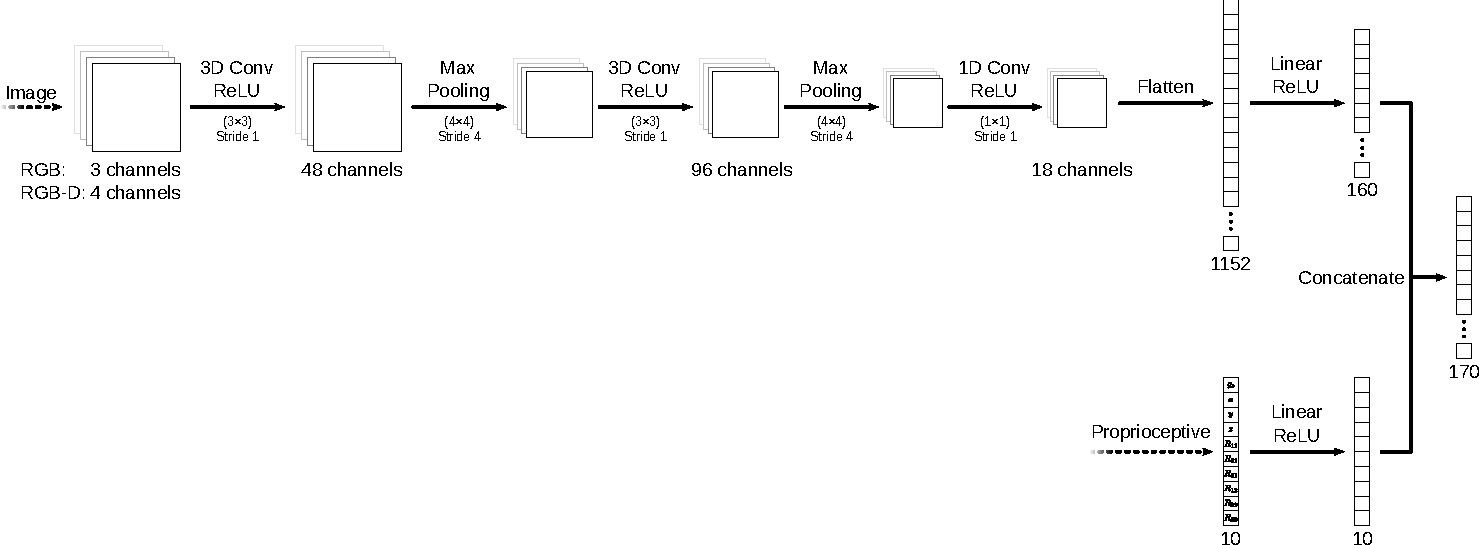
\includegraphics[width=1.0\textwidth]{experimental_evaluation/image_feature_extractor.pdf}
    \caption{Feature extractor used for RGB and RGB-D observation during experimental evaluation.}
    \label{app_fig:image_feature_extractor}
\end{figure}
